\documentclass[usenatbib]{mnras}
\usepackage[T1]{fontenc}
\usepackage[pdftex]{graphicx}
\usepackage{bm}
\usepackage{savesym}
\usepackage{amsmath}
\usepackage{amssymb}
\usepackage{algorithm}
\usepackage{algpseudocode}
\usepackage{enumitem}
\usepackage{relsize}
\usepackage{caption}
\usepackage{subcaption}
\usepackage{layouts}
\usepackage{afterpage}
\usepackage{txfonts}
\usepackage{pgf}
\usepackage{cleveref}

\newcommand{\logL}{\{ \log \Like_i \}}
\newcommand{\thetab}{\bm{\theta}}
\newcommand{\logLm}{\log \Like_\mathrm{max}}
\newcommand{\set}[1]{\{#1\}}
\newcommand{\nlive}{n_\mathrm{live}}
\newcommand{\Like}{\mathcal{L}}
\newcommand{\DKL}{D_\mathrm{KL}}



\title[Approximating the end of nested sampling]{Approximating the end of nested sampling}
\author[Z. Hu]{Zixiao Hu, Will Handley}

\begin{document}
\label{firstpage}
\pagerange{\pageref{firstpage}--\pageref{lastpage}}
\maketitle


\begin{abstract}
This project develops a technique to estimate the runtime of a nested sampling run at an intermediate iteration. The known likelihood at an iteration is fitted, then extrapolated using a Gaussian model likelihood, which allows the remaining evidence and final prior volume to be calculated. We find that the method succesfully recovers the true endpoint within standard error from the beginning for near-Gaussian likelihoods, and by the halfway point for non-Gaussian likelihoods while identifying the correct order of magnitude throughout. 
\end{abstract}

\begin{keywords}
methods: data analysis -- methods: statistical
\end{keywords}

\section{Introduction}
Nested sampling is a multi-purpose algorithm invented by John Skilling which simultaneously accomplishes the two tasks of Bayesian inference, model comparison and parameter estimation \citep{skilling}. It was immediately adopted for cosmology, and is now used in a wide range of physical sciences including particle physics, materials science \citep{physical_scientists} and machine learning \citep{split}. The core algorithm is unique for being the only algorithm which estimates high-dimensional volumes using \textit{order statistics}, which makes high-dimensional integration feasible. It also avoids problems faced by traditional Bayesian algorithms, such as multi-modality.
\par
Many instances of software for nested sampling exist, including popular implementations such as \textsc{MultiNest} \citep{multinest} and \textsc{PolyChord} \citep{polychord} which provide flexible options for nested sampling runs, as well as post-processing packages such as \textsc{anesthetic} \citep{anesthetic} to obtain and plot sample statistics. However, currently no such software is able to estimate how long a given run should last. This is of high importance to the end user, who has no indication in the middle of a run whether it will take minutes, or weeks and months to finish; even an order of magnitude estimate is useful compared to the status quo of complete ignorance.
\par
This project sets out a novel approach for estimating the endpoint of a nested sampling run at an intermediate stage. The idea is to predict the form of the likelihood function in the region we have yet to sample from, using the information we have already gained from our previous samples. We begin in section \ref{sec:Background} with an overview of Bayesian inference and nested sampling. Section \ref{sec:Endpoint prediction} presents the theory and methodology of making endpoint predictions, before results for both toy and real examples are shown in section \ref{sec:Results}. Finally, conclusions are made in section \ref{sec:Conclusions}.  


\section{Background}\label{sec:Background}
\printinunitsof{in}\prntlen{\textwidth}
We present here an overview of Bayesian inference and nested sampling; for a more detailed treatment of both subjects, we refer to \citet{sivia} as well as Skilling's original paper. 
\subsection{Bayesian inference}%
\label{sub:Bayesian inference}

Given some data $D$, Bayes' theorem tells us that the probability of some parameters $\theta$ of a model $M$ is 
\begin{equation}
	\Pr(\theta\mid D, M) = \frac{\Pr(D \mid \theta, M) \Pr(\theta \mid M)}{\Pr(D  \mid  M)}
\end{equation}
Relabelling these terms,
\begin{equation}
    P(\theta) = \frac{L(\theta) \pi(\theta)}{Z}
\end{equation}
where $\pi(\theta)$ is the \textit{prior} - what was known about a model's parameters before knowledge of the data, $P(\theta)$ is the \textit{posterior} - what is known after learning the data, and $L(\theta)$ is the \textit{likelihood} of the data given the parameters.
\par
For parameter estimation, knowledge of $L(\theta)$ and $\pi(\theta)$ is enough, but $Z$, known as the \textit{evidence}, is crucial for model comparison via Bayes factors. By definition, $Z$ is the normalisation factor 
\begin{equation}
    Z = \int L(\theta)\pi(\theta) \ d\theta
\end{equation}
which is a high-dimensional integral over the parameter space. Exponential scaling with dimension means full rasterisation is impractical for most physical applications. This motivates a sampling technique which preferentially selects for regions of high posterior mass. Traditional techniques like Markov-Chain Monte Carlo (MCMC) do not sample from the prior, so it is non-trivial to estimate the evidence from posterior samples. Nested sampling sidesteps these issues by putting the evidence first, while simultaneously yielding the posterior.



\subsection{Nested sampling}
\label{sub:Nested sampling}

We first perform a change of variable to reduce the evidence integral to a single dimension. Define the prior mass 
\begin{equation}\label{X integral}
    X(\lambda) = \int_{L(\theta)>\lambda} \pi(\theta) \ d\theta 
\end{equation}
which allows us to rewrite the evidence as 
\begin{equation}
    Z = \int_0^1 \Like(X) \ dX.
\end{equation}
The integral can be calculated by ordering the prior samples by likelihood then multiplying by the associated prior mass element. Nested sampling translates this into an algorithm which incorporates sorting \textit{de facto}, by taking a set of $\nlive$ \textit{live points} and replacing the point with the lowest likelihood with a resampled point of higher likelihood at every iteration. A choice must be made for this sampling method e.g. MCMC. The number of live points can in principle vary throughout the run, so that it depends on the iteration $k$ i.e. $n_\mathrm{live}=n_k$ \citep{dynamic_ns}. 
\par
The set of live points will therefore occupy a prior volume which tends to zero, shrinking around the maximum of the posterior. Explicit calculation of the volume $X$ within each contour is expensive, so nested sampling makes a statistical estimate using the order statistics of the remaining points: at each iteration, the volume occupied by the live points decreases by the shrinkage ratio $t$, which has probability distribution and statistics
\begin{equation}
	\Pr(t) = \nlive t^{\nlive - 1}, \quad \mathrm{E}[\log t] = -\frac{1}{\nlive}, \quad \mathrm{Var}[\log t] = \frac{1}{\nlive^2}.
\end{equation}
$X_i$ is the product of the shrinkage ratios
\begin{equation}\label{xi_formula}
    X_i = \prod_{k=0}^{i} t_k,
\end{equation}
so the $X$ themselves are also random variables. It is easier to work with $\log X$, which have the means and correlations
\begin{equation}\label{X_distribution}
	\mathrm{E}[\log X_i] = -\sum_{k=0}^{i} \frac{1}{n_k}, \quad
	\mathrm{Cov}[\log X_i, \log X_j] = \sum_{k=0}^{\mathrm{min}(i, j)} \frac{1}{n_k^2}.
\end{equation}

The evidence integral is then computed using the trapezoid rule at each step, so that
\begin{equation}
	Z = \sum_i L_i \Delta w_i = \frac{1}{2}\sum_i L_i \left( X_{i-1} - X_{i+1} \right).
\end{equation}

The algorithm terminates when the evidence in the live points falls below a user-specified fraction $\epsilon$ of the total accumulated evidence. Skilling's original paper estimates this remaining evidence $\Delta Z$ to have an upper bound of $ \Like_\mathrm{max} X_i$, while some use the average remaining likelihood. Once we have chosen to stop, the remaining evidence is included by killing the live points one by one without replacement, incrementing $Z$ as before. 
\par
The full nested sampling procedure is given in algorithm \ref{alg:ns}. 
\begin{algorithm}
\caption{Nested sampling}\label{alg:ns}
\begin{algorithmic}
\State Start with $N$ points $\theta_1, \ldots, \theta_N$ from prior
\State \hspace{\algorithmicindent} initialise $Z = 0$, $X_0 = 1$
\For{$i = 1, 2, \ldots , j$}
\State $L_i \gets \text{lowest of the current likelihood values}$
\State $X_i \gets \exp(-i/N)$
\State $w_i \gets X_{i-1} - X_i$ or $(X_{i-1} - X_{i+1})/2$
\State $Z \gets Z + L_i w_i$
\State $L_i \gets $ new point $\in \{\pi(\theta): L(\theta) > L_i\}$.
\EndFor
\State Increment $Z$ by $\langle L(\theta) \rangle X_j$.
\end{algorithmic}
\end{algorithm}

\subsection{Uncertainties and the posterior bulk}\label{subsec:Uncertainties and the posterior bulk}
\begin{figure}
\begin{center}
	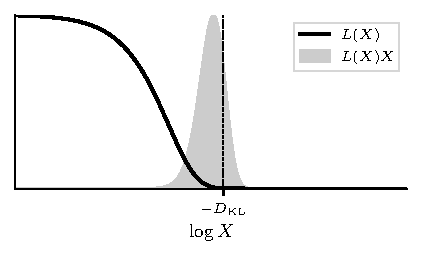
\includegraphics[scale=]{Figures/LX.pdf}
\end{center}
\caption{Plot showing the likelihood and the posterior weights $\Like(X)X$. The bulk of posterior mass is contained within a region of size $e^{-\DKL}$, meaning one must iterate through at least $n\DKL$ steps to fully explore the posterior.}
\label{fig:LX}
\end{figure}

\begin{figure}
\begin{center}
	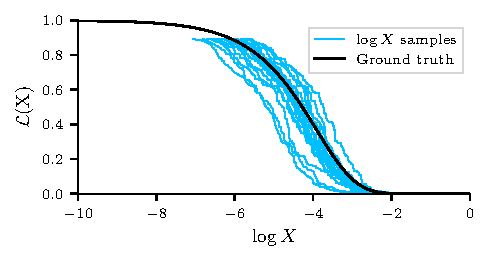
\includegraphics[scale=]{Figures/X_samples.pdf}
\end{center}
\caption{Plot showing samples of $\log X$ plotted against the likelihoods of the sample points. The uncertainty increases with the number of steps taken.}
\label{fig:X_samples}
\end{figure}


Most of the posterior is contained within a small fraction of the prior of size $X^{*} = e^{-\DKL}$, where
\begin{equation}
\DKL = \int P(\theta) \log  \frac{P(\theta)}{\pi(\theta)} \ d\theta
\end{equation}
is the information gain between the prior and posterior; this is visualised in figure \ref{fig:LX}. To learn anything about the posterior or calculate an accurate evidence, we must compress down to this volume. 
\par
From equation \eqref{X_distribution}, it is easy to see that for a constant number of live points $n$ $\log X$ follows Poisson statistics:
\begin{equation}
	\mathrm{E}[\log X_i] = - \frac{i}{n}, \quad \mathrm{Var}[\log X_i] = \frac{i}{n^2}.
\end{equation}
This is illustrated in figure \ref{fig:X_samples}, where samples are taken from the $X$ distribution and plotted against the likelihood values. To reach the posterior bulk we must therefore take $i^{*} = n\DKL$ steps, which translates to an uncertainty in $\log X^{*} = -\DKL \pm \sqrt{\DKL/n}$. The evidence is $Z = \langle \Like \rangle X^{*}$, or
\begin{equation}
\log Z = \langle \log \Like \rangle + \log X^{*}.
\end{equation}
The first term has low error, since the only difference that errors in $X$ makes is to slightly change the region we average over. Uncertainties in $\log Z$ are therefore dominated by the $\mathcal{O}(1/\sqrt{n})$ errors on $\log X_i$, which are much more significant than the $\mathcal{O}(n^{-2})$ quadrature errors.
\par
The next section will outline the methodology for making endpoint predictions.


\section{Endpoint prediction}\label{sec:Endpoint prediction}
We shall begin by discussing a simple ``eyeball" method for making predictions that is familiar to experienced users of nested sampling, which makes a good sanity check to compare to the more principled approach.
\subsection{Eyeball method}
At an intermediate iteration of a nested sampling run, the output might look something like that shown in the first two columns of table \ref{tab:ns_output}. 
\begin{figure}
\centering
\scalebox{0.9}{\begin{tabular}{|c|c|c|}
\hline
iteration & log Z  & $d\log Z$   \\
\hline
6000 & -34.481 & 1.317 \\ 
6200 & -32.606 & 1.875 \\ 
6400 & -30.700 & 1.906 \\ 
6600 & -29.008 & 1.692 \\ 
6800 & -27.416 & 1.591 \\ 
7000 & -25.865 & 1.551 \\ 
7200 & -24.449 & 1.416 \\ 
7400 & -23.034 & 1.415 \\ 
7600 & -21.617 & 1.417 \\ 
7800 & -20.267 & 1.349 \\ 
8000 & -18.950 & 1.317 \\
\hline
\end{tabular}}
\captionof{table}{Output of accumulated log-evidence during a nested sampling run.}
\label{tab:ns_output}
\end{figure}
\begin{figure}
  \centering
  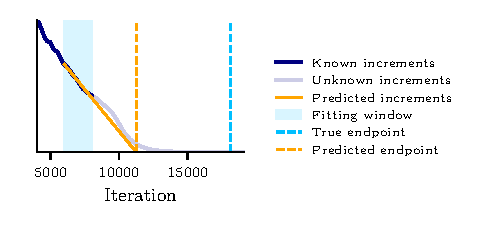
\includegraphics{Figures/linear_extrapolate.pdf}
  \captionof{figure}{Prediction of endpoint using linear extrapolation. The estimate is much lower than the true endpoint, primarily because of the long tail in $d\log Z$.}
  \label{fig:linear_extrapolate}
\end{figure}
The outputs $\log Z$ appear to converge at a predictable rate, which is shown in terms the increments in column three. One could feasibly extrapolate these to predict when the increments approach zero, which gives an iteration number for convergence. 
\par
This is shown for a linear extrapolation in figure \ref{fig:linear_extrapolate}. The prediction is clearly an underestimate, which is mainly due to the nonlinear profile of $d\log Z$ having a long tail. However, this makes a good benchmark to beat for the more principled method using likelihood approximation. 

\subsection{Likelihood approximation method}
We want to make an estimate of the number of iterations until the termination condition is met, which is when the remaining evidence falls below a fraction $\epsilon$ of the accumulated evidence.
Predictions can be made ahead of time because of the live points, which are sampled from higher likelihood regions that we have not yet compressed to. It is important to note that there will always be a small region which the live points do not penetrate because they are too diffuse, which can be seen in figure \ref{fig:dead_live_points}. 
\begin{figure}
\begin{center}
	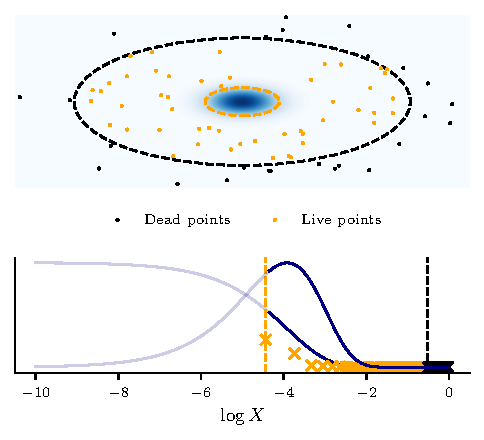
\includegraphics[scale=]{Figures/dead_live_points.pdf}
\end{center}
\caption{Plots showing the state of a nested sampling at an intermediate iteration. The live points are samples from higher likelihood regions, which allow us to see the remaining likelihood ahead of time. However, there is always a small high likelihood region where we have no samples, simply because the live points are too diffuse.}
\label{fig:dead_live_points}
\end{figure}
\par
If we could estimate the form of $\Like(X)$ at the higher likelihoods in terms of some \textit{likelihood model} $f(X, \thetab)$, we would be able to express the prior volume $X_f$ which we need to compress to as
\begin{equation}
	\Delta Z = \epsilon Z_\mathrm{tot},
\end{equation}
\begin{equation}\label{model endpoint}
	\int_0^{X_f} f(X, \thetab)\ dX = \epsilon \left( \int_0^{X_i} f(X, \thetab)\ dX + Z_\mathrm{dead} \right),
\end{equation}
where $X_i$ is the volume of the iteration we have currently compressed to, and $Z_\mathrm{dead}$ is the evidence we have accumulated up to this point. $X_f$ can then be identified by solving the above equation either analytically or numerically. Remembering that at each iteration $\log X$ decreases by $1/\nlive$, the total number of iterations $N_f$ will be
\begin{equation}
	N_f = - \nlive \log X_f .
\end{equation}

\subsubsection{Model choice}\label{sec:Model choice}
The choice of the model $f(X, \thetab)$ serves two purposes; to \textit{smooth} over the stochasticity in the live points, since $\Like(X)$ is typically a smooth function, and more importantly to \textit{extrapolate} into the region where we have no samples.
\par
Making this extrapolation necessitates assumptions about the form of the likelihood in the unsampled region. It is sensible to assume it is guided by what came before it, so we fit the model on the known likelihods of the live and dead points. Apart from this, we should make the model $f(X, \thetab)$ as flexible as possible to extrapolate without bias. We chose the model to be a Gaussian with freely varying parameters $\thetab = (\Like_\mathrm{max}, d, \sigma)$:
\begin{equation}
	f(X, \thetab) = \Like_\mathrm{max} \exp\left(-\frac{X^{2/d}}{2\sigma^2}\right).
\end{equation}
The choice was made because it is analytically tractable, and because many likelihoods in practice are near-Gaussian at their peaks. Allowing $d$ to vary freely increases flexibility, and reflects the fact that while the dimensionality of the posterior is fixed, the equivalent dimension for a Gaussian of the same information content can differ \citep{Handley_2019}.


\subsubsection{Endpoint formula}
Now we are equipped with the tools to make endpoint predictions. We will begin by fitting the model over the live points only. At each iteration, estimate the prior volumes of the live points to be those which correspond to killing off each point one by one without replacement and using formula \eqref{X_distribution}. Combined with the live likelihoods $\logL$, the parameters of the model can be found by minimising the cost function
\begin{equation}\label{chi squared}
	C^2(\thetab) = \sum_i \left| \log \Like_i - \log f(X_i, \thetab) \right| ^2
\end{equation}
with respect to $\thetab$. A key feature is that we can analytically differentiate  $C^2$ for the Gaussian model, which allows us to write the optimal values of $\logLm$ and $\sigma$ in terms of the optimal values of $d$:
\begin{equation}
    \sigma^2 = \frac{N \sum_i X_i^{4/d} - \left(\sum_i X_i^{2/d}\right)^2}{2 \sum_i \log \Like_i \sum_i X_i^{2/d} - 2N \sum_i \log \Like_i X_i^{2/d}}
\end{equation}
\begin{equation}
    \logLm = \frac{1}{N} \sum_i \logL + \frac{1}{2N\sigma^2} \sum_i X_i^{2/d} 
\end{equation}
(where $N$ here is the number of data points in we fit over), and simply minimise with respect to $d$ instead of all three variables. The result is that we are able to consistently find \textit{global} rather than local minima in a single optimisation run. We do not need to concern ourselves with the usual difficulties of global optimisation like comparing an ensemble of initial conditions, which is orders of magnitude slower.
\par
Once we have obtained the best-fit $\thetab$, the endpoint can be calculated in the manner described in \eqref{model endpoint};
\begin{equation}
	\epsilon = \frac{\int_0^{X_f} \Like_\mathrm{max} \exp\left(-X^{2/d}/2\sigma^2\right)\ dX}{\int_0^{X_i} \Like_\mathrm{max} \exp\left(-X^{2/d}/2\sigma^2\right)\ dX + Z_\mathrm{dead}}.
\end{equation}
The integrals have the analytic solution
\begin{equation}
	\int_0^{X_k} \Like_\mathrm{max} \exp\left(-X^{2/d}/2\sigma^2\right)\ dX = \frac{d}{2} \cdot 2^{d/2} \cdot \sigma^{d} \cdot \gamma_k
\end{equation}
where $\gamma_k = \gamma\left(d/2, X_k^{2/d}/2\sigma^2\right)$ is the lower incomplete gamma function. After taking the inverse of  $\gamma$ and a few more steps of algebra, we arrive at
\begin{multline}
	\log X_f = \frac{d}{2}\log 2 + d \log \sigma \\
	+ \log \gamma^{-1} \left( d/2 ,\ \epsilon \left(\gamma_i+ 2^{-d/2} \sigma^{-d} Z_\mathrm{dead}/\Like_\mathrm{max}\right)\right),
\end{multline}
and $N_f$ is just  $-\nlive$ multiplied by this. 
\par
An useful feature is that the formula is robust when we are far away from the posterior bulk. In this phase, the inferred values of $\Like_\mathrm{max}$ turn out to be very uncertain and often divergent, but the dead evidence is also negligible, so $\Like_\mathrm{max}$ has little impact on the prediction. Once $Z_\mathrm{dead}$ becomes comparable to the live evidence $\Like_\mathrm{max}$ does begin to impact the prediction, but at this point we have reached the posterior bulk, so we expect $\Like_\mathrm{max}$ to be well-estimated and thus contribute in a useful way.
\par
Note that the prediction procedure should not contribute any significant time complexity to the nested sampling run, since it involves no likelihood evaluations. 

\subsubsection{Uncertainties}
Our lack of knowledge about the unsampled region means that there is always the chance that there is some huge likelihood spike at small $X$. Since there is no way to anticipate this, all uncertainty estimates are underestimates in the sense that they cannot account for this possibility; there is no estimate which will \textit{always} include the true endpoint. 
\par
We will therefore restrict ourselves to quantifying the uncertainties associated with how we have modelled the \textit{known} data, remembering that because of our lack of knowledge, the true endpoint may fall significantly outside of this range. These uncertainties have two sources: the variance in the prior volume estimates, and the uncertainty in the least squares minimisation. Since the former is the main error in nested sampling, we expect it to dominate. As we saw in section \ref{subsec:Uncertainties and the posterior bulk}, different sets of $\set{X_i}$ drawn from its probability distribution lead to different "maps" of what the remaining likelihood looks like, which lead to different endpoint predictions. The natural way to handle this is to sample from $\Pr(\bm{X})$ then find the best-fit  $\thetab$ and endpoint for each sample, from which we can obtain the mean and variance in the estimates. An visualisation of this approach is shown in figure \ref{fig:gauss_overfit}.

\begin{figure}
\begin{center}
	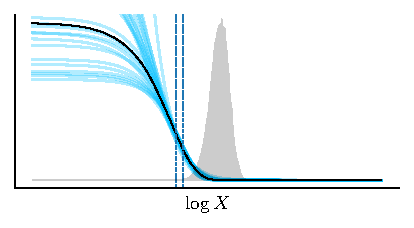
\includegraphics[scale=]{Figures/gauss_overfit.pdf}
\end{center}
\caption{Plot showing fits of the likelihood corresponding to different draws of $\log X$. The different realisations of the likelihood lead to a set of endpoint predictions, from which a mean and variance can be obtained.}
\label{fig:gauss_overfit}
\end{figure}




\section{Results}\label{sec:Results}
\subsection{Toy data}
Let us now apply the methodology developed above in practice. We consider the following toy examples:
\begin{enumerate}[leftmargin=0.3in, label=(\alph*)]
	\item A spherically symmetric Gaussian, $\log \Like = -|\bm{r}|^2/2\sigma^2$ in $d$ dimensions
	\item A discontinous "wedding cake" likelihood with Gaussian profile and parameter $\alpha_\mathrm{w}$ controlling the plateau depth, as presented in \cite{plateaus} and shown in figure \ref{fig:wedding_3d}.
	\item A Cauchy likelihood $\log \Like = - \frac{1 + d}{2} \log (1 + |\bm{r}|^2/\gamma^2)$.
\end{enumerate}
\begin{figure}
\begin{center}
	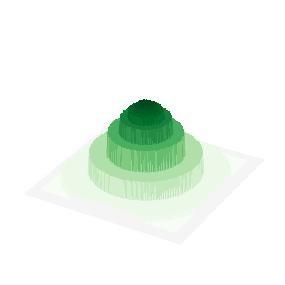
\includegraphics[scale=]{Figures/wedding_3d.pdf}
\end{center}
\caption{An example ``wedding cake" likelihood which has plateaus on top of a Gaussian profile}
\label{fig:wedding_3d}
\end{figure}

Parameters were chosen to have large values of $\DKL$, which are more difficult to model due to the large distance to the posterior bulk.
\par
Nested sampling runs were made for the above likelihoods for $\nlive = 500$ (plots for different numbers of live points are not shown here, but the results are broadly the same). The state at each iteration (i.e. the likelihoods of the dead and live points) was then extracted using \textsc{anesthetic}. At each iteration, the model is fitted over a number of points determined by the bandwidth selection procedure outlined above. For the error bars, we draw an \textit{ensemble} of 25 $\bm{X}$ samples from the distribution \eqref{xi_formula}, and find the optimal $\thetab$ and corresponding  $N_f$ for each sample to get the mean and variance of the prediction. 
\par
Results are shown in figure \ref{fig:toy_predictions}. For all cases, the predictions become more accurate as the iteration increases because the samples shrink around and eventually cross the posterior bulk, leading to an increasingly representative picture of the posterior. The method works very well for the first two likelihoods, recovering the correct endpoint within standard error for the entire run. This is expected, since the model likelihood has the same form as the true likelihoods, so one expects the extrapolation made to be accurate even when we are far away from the posterior bulk.
\par
The Cauchy likelihood shows the result when this is not the case; without samples in the bulk, a Gaussian extrapolation performs poorly. However, the correct order of magnitude is still obtained, which is a significant improvement on the status quo of complete ignorance. 
\begin{figure*}
\begin{center}
	\subfloat[Gaussian: $d = 30$, $\sigma = 0.01$, $\DKL = 84$]{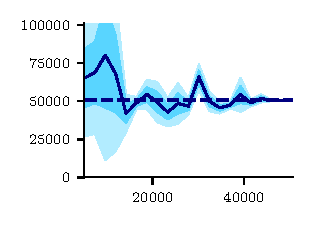
\includegraphics[scale=]{Figures/gauss_predictions.pdf}}
	\subfloat[\centering Wedding cake: $d = 20$, $\sigma = 0.001$, $\alpha_\mathrm{w}=0.5$, $\DKL = 93$]{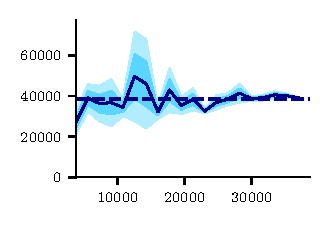
\includegraphics[scale=]{Figures/wedding_predictions.pdf}}
	\subfloat[Cauchy: $d = 10$, $\gamma = 0.0001$, $\DKL = 48$]{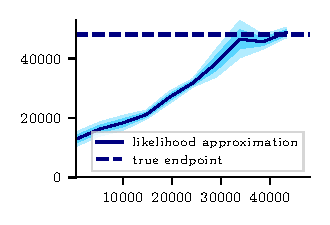
\includegraphics[scale=]{Figures/cauchy_predictions.pdf}}
\end{center}
\caption{Plot showing endpoint predictions for the toy likelihoods. The mean estimate is dark blue, while the shading shows the $1\sigma$ and $2\sigma$ uncertainties. For the first two likelihoods (which have Gaussian profile), the true endpoint falls within error for practically all of the run. The Cauchy likelihood is less well-estimated because it is highly non-Gaussian, with the true endpoint outside the reasonable uncertainty range but in the correct order of magnitude.}
\label{fig:toy_predictions}
\end{figure*}

\subsection{Real data}
The model was tested on real nested sampling runs for quantification of cosmological parameter tensions. Results are shown in figure \ref{fig:lcdm_predictions}, with the likelihood approximation method compared against the benchmark.
\par
The likelihood model clearly performs better. For all of the chains, the true endpoint was recovered within arund standard error by the halfway point, and falls within the correct order of magnitude throughout all of the runs. In comparison, the benchmark model mostly failed to get the correct order of magnitude on the number of iterations remaining, especially near the end of each run.
\par
Furthermore, the first four likelihoods are highly non-Gaussian, which validates the choice of a Gaussian likelihood model. For all chains, further work needs to be done to place a more accurate upper bound on the prediction uncertainty at early iterations. 
\begin{figure*}
\begin{center}
	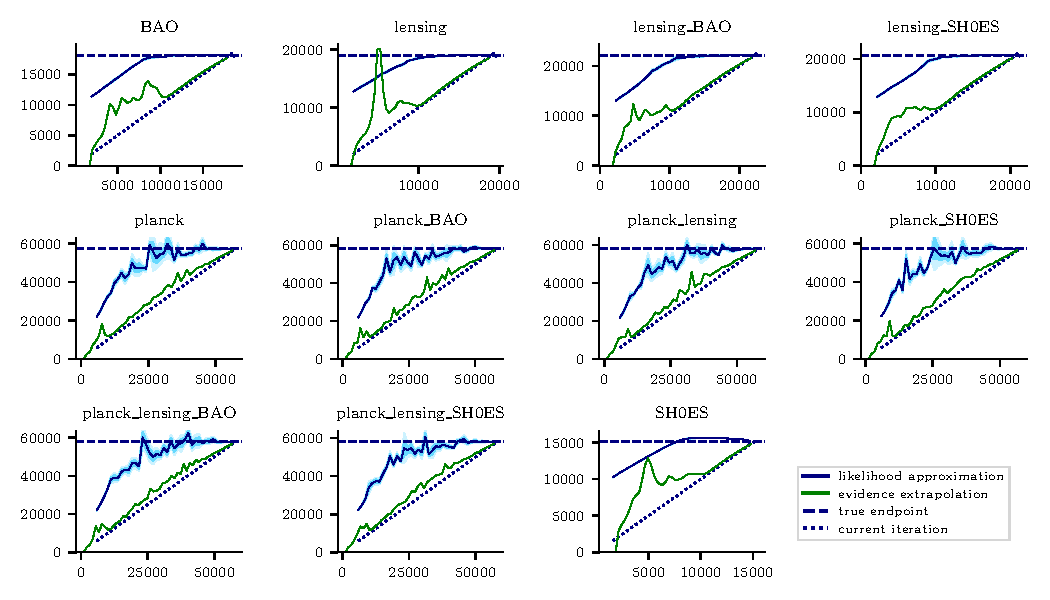
\includegraphics[scale=]{Figures/lcdm_predictions.pdf}
\end{center}
\caption{Plots showing the endpoint predictions for the benchmark model as well as the likelihood approximation model. The likelihood model visibly performs better, managing to recover the true endpoint within around standard error at the halfway point for all the chains. The first four likelihoods are highly non-Gaussian, which validates the choice of a Gaussian model.}
\label{fig:lcdm_predictions}
\end{figure*}




\section{The anatomy of a Gaussian}

In general, it is well known (to those who know such things) that the anatomy of a Gaussian says that
\begin{equation}
    \boxed{\log\mathcal{L}_\mathrm{max} = \langle\log\mathcal{L}\rangle_\mathcal{P} + \frac{d}{2}},  \qquad \boxed{\mathrm{var}(\log\mathcal{L})_\mathcal{P} = \frac{d}{2}},
\end{equation}
namely the posterior average of the log likelihood is $d/2$ less than the maximum, and the variance of the loglikelihood over the posterior is $\frac{d}{2}$. Whilst this is exact for gaussians, this provides a good rule of thumb for other distributions. 

For example, one may use this to explain why MCMC sampling is a very bad way to maximise, since even in the limit of a very large number of samples from the posterior $n$, the largest of these will be within a few $\sqrt{\frac{d}{2}}$ standard deviations of the mean, and therefore very far away from the maximum $\frac{d}{2}$ away.\footnote{TODO: can we do some analytics on the MCMC eaxmple as well?}

The same is true for nested sampling, although since it is not a posterior sampler, but a likelihood upward scanner, the argument is a little more subtle, which we work through below.



We will work with a Gaussian loglikelihood, lengthscale $\sigma$, defined in terms of prior volumes $0<X<1$
\begin{equation}
    \log\mathcal{L}
    =\log\mathcal{L}_\mathrm{max} - \frac{1}{2\sigma^2}X^{2/d}
    =\log\mathcal{L}_\mathrm{max} - \frac{1}{2\sigma^2}\exp\left(\frac{2}{d}\log X\right).
    \label{eq:LX}
\end{equation}
We will assume the run has progressed far enough so that prior effects may be neglected, and that $\sigma\ll 1$ is sufficiently small that for the arguments below edge effects may be neglected.

Note that from the Gaussian profile we can see that as $\log X\to-\infty$ at a steady rate of compression, we approach the maximum loglikelihood exponentially slowly, with an decay rate of $\frac{d}{2}$

Taking $X \sim e^{-i/n}$ we see this as
\begin{equation}
    \log\mathcal{L} = \log\mathcal{L}_\mathrm{max} - \exp\left(-\frac{i-i_0}{nd/2}\right), \qquad i_0 = -\frac{nd}{2}\log 2\sigma^2
\end{equation}
in principle this converges very quickly, although never quite reaches the maximum.

\section*{The anatomy of a gaussian}
\begin{equation}
    P(\log\mathcal{L}) = \frac{1}{\Gamma(\frac{d}{2})}e^{\log\mathcal{L}-\log\mathcal{L}_\mathrm{max}} (\log\mathcal{L}_\mathrm{max}-\log\mathcal{L})^{\frac{d}{2}-1}
\end{equation}
i.e. $2(\log\mathcal{L}_\mathrm{max}-\log\mathcal{L})\sim \chi^2_{d} $

\section*{Observation 1: the largest likelihood live point}
Assume we are at an iteration such that $\mathcal{L}_*$ is the current likelihood contour (i.e. the likelihood of the dead point we have just deleted), and that we have $n$ live pointsdistributed uniformly in prior volume beneath this. 
Since the the live points are distributed in prior volume up to $X_*$, $P(X) = [0<X<X_*]$,
Inverting \cref{eq:LX} we may show that the distribution of loglikelihoods is
\begin{equation}
    P(\log\mathcal{L}) = \frac{d}{2}\frac{(\log\mathcal{L}_\mathrm{max}-\log\mathcal{L})^{\frac{d}{2}-1}}{(\log\mathcal{L}_\mathrm{max}-\log\mathcal{L}_*)^{\frac{d}{2}}}[0<\log\mathcal{L}<\log\mathcal{L}_*].
    \label{eq:PL}
\end{equation}
It is helpful at this stage therefore to define a parameter
\begin{equation}
    y = \frac{\log\mathcal{L}-\log\mathcal{L}_*}{\log\mathcal{L}_\mathrm{max}-\log\mathcal{L}_*} \qquad\Leftrightarrow\qquad \log\mathcal{L} = y\log\mathcal{L}_\mathrm{max} + (1-y)\log\mathcal{L}_*
    \label{eq:y}
\end{equation}
as a normalised likelihood with $y=0$ corresponding to $\mathcal{L}=\mathcal{L}_*$ and $y=1$ to $\mathcal{L}=\mathcal{L}_\mathrm{max}$, which has distribution
\begin{equation}
    P(y) = \frac{d}{2}(1-y)^{\frac{d}{2}-1}[0<y<1].
    \label{eq:Py}
\end{equation}
We now seek the distribution of the largest likelihood $\log{\mathcal{L}}_\mathrm{max}^\mathrm{live}$ (or equivalently the largest ${y}_\mathrm{max}^\mathrm{live}$) in the set of $n$ live points. We first integrate to find the CDF
\begin{equation}
    P(y<Y) = 1-(1-Y)^{\frac{d}{2}}[0<Y<1].
    \label{eq:Py}
\end{equation}
note that to find the largest of $n$ independent variables we simply multiply 
\begin{equation}
    P(y_1,y_2,\ldots<Y) = (1-(1-Y)^{\frac{d}{2}})^n[0<Y<1].
    \label{eq:Py}
\end{equation}
and then differentiate with respect to $Y$ to find the PDF for largest likelihood in the live points
\begin{equation}
    P(y_\mathrm{max}^\mathrm{live}) = \frac{nd}{2}(1-y_\mathrm{max}^\mathrm{live})^{\frac{d}{2}-1}\left(1-(1-y_\mathrm{max}^\mathrm{live})^{\frac{d}{2}}\right)^{n-1}[0<y_\mathrm{max}^\mathrm{live}<1],
    \label{eq:Pyhat}
\end{equation}
which may be roughly summarised as:
\begin{equation}
    y_\mathrm{max}^\mathrm{live} \sim 1-\frac{\Gamma(1+\frac{2}{d})\Gamma(1+n)}{\Gamma(1+\frac{2}{d}+n)} \pm \left( \frac{\Gamma(1+n)\Gamma(1+\frac{4}{d})}{\Gamma(1+\frac{4}{d}+n)} - \frac{\Gamma(1+\frac{2}{d})^2 \Gamma(1+n)^2}{\Gamma(1+\frac{2}{d}+n)^2}\right)^{\frac{1}{2}},
    \label{eq:ymax}
\end{equation}
or in the large $d$, $n$ limit
\begin{align}
    \lim_{d\to\infty} y_\mathrm{max}^\mathrm{live} &\sim \frac{2H_n}{d} \pm \left(\frac{2(\pi^2 - 6\Psi^{(1)}(1+n))}{3d^2}\right)^{\frac{1}{2}},
    \label{eq:ymaxd}\\
    \lim_{d,n\to\infty} y_\mathrm{max}^\mathrm{live} &\sim \frac{2\log n}{d} \pm \sqrt{\frac{2}{3}}\frac{\pi}{d},
    \label{eq:ymaxdn}
\end{align}
where $\psi^{(1)}$ is the trigamma function and $H_n$ is the $n$th harmonic number.

This shows that in general the live points are nowhere near the maximum loglikelihood at any iteration, though they do steadily squeeze the interval $[\log\mathcal{L}_*,\log\mathcal{L}_\mathrm{max}]$. In particular, in high dimensions $n$ only gets us harmonically/logarithmically closer, whilst $d$ pushes us linearly further away. Our end result is that:
\begin{equation}
    \boxed{
        \log{\mathcal{L}}_\mathrm{max}^\mathrm{live} \approx \log\mathcal{L}_\mathrm{max} - (1-y_\mathrm{max}^\mathrm{live})(\log\mathcal{L}_\mathrm{max}-\log\mathcal{L}_*)
    },
\end{equation}
where you may take any of the $y_\mathrm{max}^\mathrm{live}$ expressions above from \cref{eq:ymax,eq:ymaxd,eq:ymaxdn}.

We may also rewrite the distribution \cref{eq:Pyhat} without $y$ to give
\begin{equation}
    \frac{\log\mathcal{L}_\mathrm{max}^\mathrm{live}-\log\mathcal{L}_*}{\log\mathcal{L}_\mathrm{max}-\log\mathcal{L}_*}
\end{equation}
\begin{equation}
    P(\log\mathcal{L}_\mathrm{max}^\mathrm{live}) = \frac{nd}{2}(\log\mathcal{L}_\mathrm{max} - \log\mathcal{L}_\mathrm{max}^\mathrm{live})^{\frac{d}{2}-1}\left((\log\mathcal{L}_\mathrm{max}-\log\mathcal{L}_*)^{\frac{d}{2}}-(\log\mathcal{L}_\mathrm{max} - \log\mathcal{L}_\mathrm{max}^\mathrm{live})^{\frac{d}{2}}\right)^{n-1}[0<y_\mathrm{max}^\mathrm{live}<1],
\end{equation}

\subsection*{Observation 2: the termination contour $\mathcal{L}_\mathrm{end}$}

One strategy for terminating nested sampling is to halt when the amount of evidence in the live points is some fraction $f$ of the amount of total evidence (or evidence in the dead points). Providing $f\ll 1$, then this is approximately the same as the fraction of evidence left above likelihood contour $\mathcal{L}_\mathrm{end}$:
\begin{equation}
    f = \frac{\int_0^{X_\mathrm{end}} \mathcal{L} dX}{\int_0^\infty \mathcal{L} dX}.
    \label{eq:fint}
\end{equation}
Note that we have assumed that prior effects are negligible (so $1=\infty$).
Computing this for \cref{eq:LX} we find the answer in terms of lower incomplete gamma functions
\begin{equation}
    f = 1- \frac{\Gamma_{d/2}(\frac{X_\mathrm{end}^{2/d}}{2\sigma^2})}{\Gamma(\frac{d}{2})}.
    \label{eq:f}
\end{equation}
Taking the $X_\mathrm{end}\ll (\sqrt{2}\sigma)^d$ limit (almost certainly valid at termination) we find
\begin{equation}
    \lim_{X_\mathrm{end}\ll (\sqrt{2}\sigma)^d} f \approx \frac{X_\mathrm{end}}{(\sqrt{2}\sigma)^d\Gamma(1+\frac{d}{2})} = \frac{(\log\mathcal{L}_\mathrm{max}-\log\mathcal{L}_\mathrm{end})^{\frac{d}{2}}}{\Gamma(1+\frac{d}{2})}.
\end{equation}
We thus have an expression relating $\mathcal{L}_\mathrm{end}$ at termination to the termination fraction $f$. This becomes yet more pleasing in the large $d$ limit, since $f^{2/d}\to 1$, we find via a stirling/Stirling approximation:
\begin{equation}
    \lim_{d\to\infty} \log\mathcal{L}_\mathrm{end} \approx \log\mathcal{L}_\mathrm{max} - \frac{d}{2e}.
\end{equation}
In the event that we keep $f$ in, we replace $\frac{d}{2e}\to \frac{d}{2e}f^{2/d}$, so we can of course battle the $\frac{d}{2e}$ term, but this becomes exponentially difficult in high dimensions.

\subsection*{Observation 3: nested sampling as a maximiser}

Putting this together, taking $\mathcal{L}_*$ in \cref{eq:y} to be $\mathcal{L}_\mathrm{end}$, and combining this with the large $d,n$ limit of \cref{eq:ymaxdn} we find
\begin{equation}
    \boxed{
        \log{\mathcal{L}}_\mathrm{max}^\mathrm{live} \approx \log\mathcal{L}_\mathrm{max} - \frac{d}{2e} + \frac{\log n}{e} \pm \frac{\pi}{\sqrt{6}e}
    },
\end{equation}
showing that in general the anatomy that nested sampling will finish at a contour $\frac{d}{2e}$ away from the maximum loglikelihood, and the final set of $n$ live points can get you $\frac{\log n}{2e}$ closer, with a chance of getting $\sim\frac{\pi}{\sqrt{6}e}=0.472$ closer still by statistical fluctuation.

\begin{figure*}
\begin{center}
	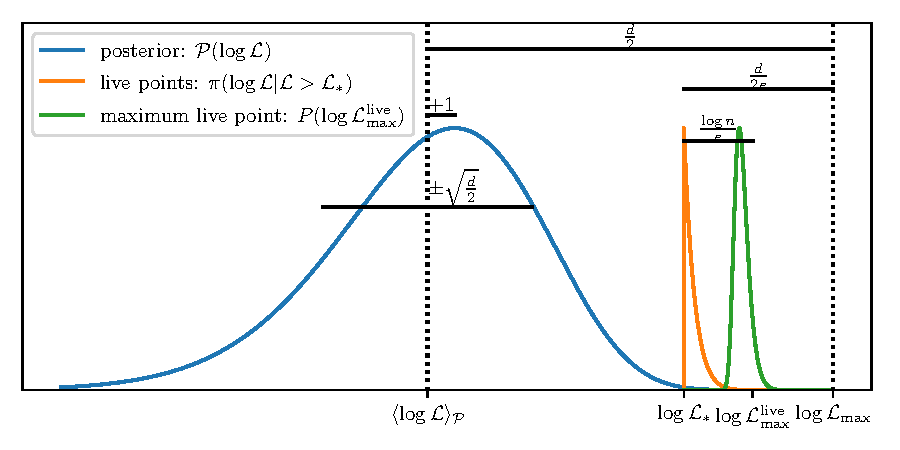
\includegraphics{Figures/anatomy.pdf}
\end{center}
\caption{}
\label{fig:anatomy}
\end{figure*}

\section{Conclusions}\label{sec:Conclusions}
In this project we have developed a model to estimate the endpoint of a nested sampling run, which has no precedent in the literature. This was done by predicting the form of the likelihood in the region that the samples have not reached, via fitting of a Gaussian model likelihood to the points already known to us. Assuming that the likelihood continues in a similar trajectory leads to an estimate of the remaining evidence, and hence the end iteration.  
\par
The approach taken was shown to be highly successful for near-Gaussian likelihoods, finding the true endpoint within error from the start of the run; this was expected, because the form of the model matched the likelihood. For a Cauchy likelihood as well as the real nested sampling runs that were tested, the estimates were less accurate, but still able to find the correct order of magnitude which is useful to the end user. Furthermore, the correct endpoint was able to be recovered within standard error at the halfway point of the runs.
\par
Two main refinements are recommended: the uncertainty quantification should be expanded to include the true endpoint from the beginning of the run, and the analysis should be extended to include the iteration prediction when the number of live points is allowed to vary, so that endpoints can be estimated for dynamic nested sampling.

\section*{Data availability}
The data and code for the project can be found in the repository \url{https://github.com/zixiao-h/aeons}.

\bibliographystyle{mnras}
\bibliography{references}


\label{lastpage}
\end{document}
